Hasta este momento, hemos utilizado el marco web Actix para proporcionar vistas básicas. Sin embargo, esto solo puede llevarnos hasta cierto punto cuando se trata de extraer datos de la solicitud y devolverlos al usuario.

\section{Conociendo la configuración inicial}
En la figura \ref{cap3:001} se observa la estructura de la tienda.
 
\begin{figure}[htb]
	\centering
	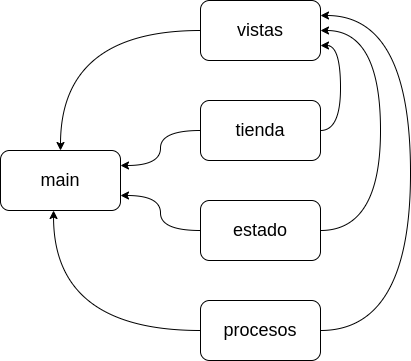
\includegraphics[width=0.5\textwidth]{capitulo3/estru_tienda.png}
	\caption{Estructura básica de la tienda}
	\label{cap3:001}
\end{figure}

Aquí, registraremos todos los módulos en el archivo principal y luego colocaremos todos estos módulos en las vistas que se utilizarán. Básicamente, estamos intercambiando la interfaz de línea de comandos, Diseño de su aplicación web en Rust, con vistas web. La combinación de estos módulos nos da los siguientes archivos en el código base:

\begin{figure}[htb]
	\centering
	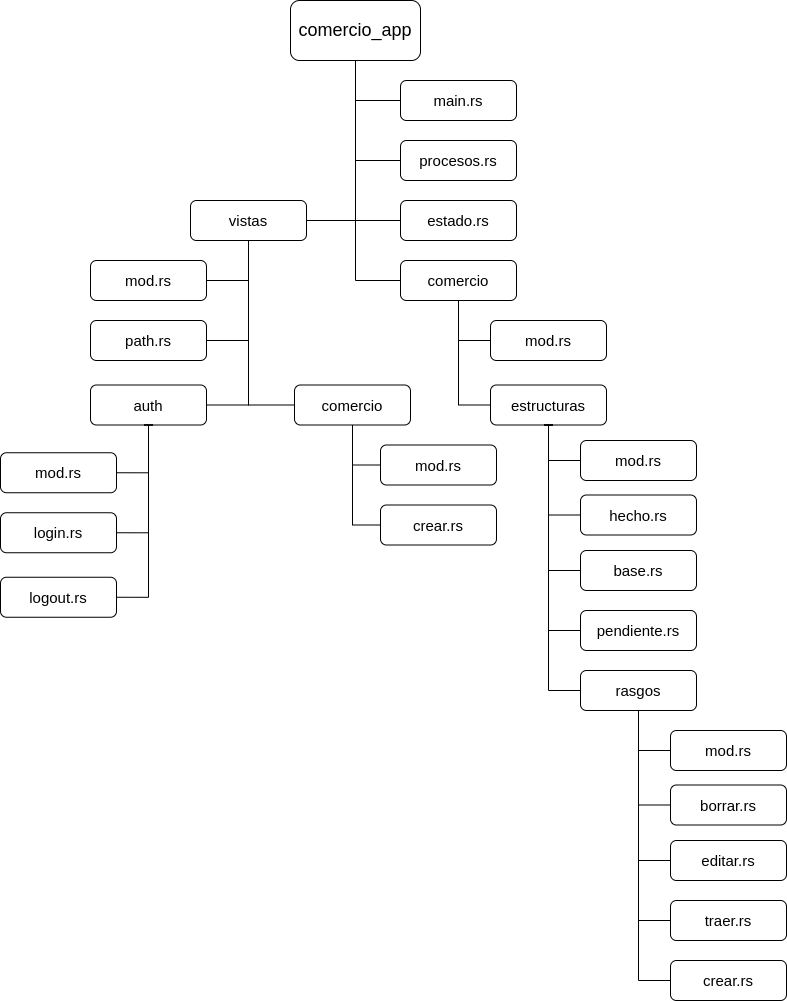
\includegraphics[width=0.5\textwidth]{capitulo3/estru_archivo.png}
	\caption{Estructura básica de los archivos de la tienda}
	\label{cap3:002}
\end{figure}

Tenga en cuenta que aunque estamos agregando módulos, hay un archivo que será nuevo para nosotros, y este es \textbf{main.rs}. Aquí, tenemos un código cruzado que estamos empalmando:

\begin{lstlisting}[language=C]
use actix_web::{App, HttpServer};
mod estado;
mod procesos;
mod comercio;
mod vistas;


#[actix_rt::main]
async fn main() -> std::io::Result<()> {
	HttpServer::new(|| {
		let app = App::new().configure(
		vistas::fabrica_vistas);
		return app})
	.bind("127.0.0.1:8000")?
	.run()
	.await	
}
\end{lstlisting}

Aquí, definimos los módulos y luego definimos nuestro servidor. Debido a que el servidor utiliza \textbf{fabrica\_vistas}, no tendremos que modificar este archivo durante el resto de este capítulo. En su lugar, encadenaremos las funciones de fábrica que se llamarán en la función \textbf{fabrica\_vistas}.

En este punto, podemos sentarnos y apreciar los dividendos de todo el arduo trabajo que hicimos en los capítulos anteriores. El aislamiento de principios y módulos bien definidos nos permitió insertar nuestra lógica desde nuestro programa de línea de comandos en nuestra interfaz de servidor con un esfuerzo mínimo. Ahora, todo lo que tenemos que hacer es conectarlo a nuestro módulo de vistas y luego pasar parámetros a esas vistas.

\section{Pasando parámetros}

Ahora que estamos familiarizados con las vistas básicas, vamos a pasar parámetros y datos a la vista. Nuestro módulo de vistas de comercio tendrá la estructura que se muestra en la rama izquierda de la figura \ref{cap3:002}.

Para demostrar esto, vamos a construir una vista básica que toma un parámetro de la \textbf{URL} y crea un elemento de tarea. Para ello, tendremos que hacer lo siguiente:

\begin{itemize}
	\item Cargue el estado actual de la lista de personas pendientes.
	\item Obtenga el título del nuevo elemento pendiente de la URL.
	\item Pase el título y la cadena pendiente a través de \textbf{fabrica\_comercio}.
	\item Pase el resultado del paso anterior, junto con la cadena de creación y el estado, a la interfaz del módulo de proceso.
	\item Devuelve una cadena al usuario para indicar que el proceso ha finalizado.
\end{itemize}


Debido a que el proceso anterior consiste principalmente en interactuar con interfaces de módulos cuidadosamente empaquetadas, todo esto se puede lograr con esta función simple, que se puede encontrar en el archivo \textbf{vistas/comercio/crear.rs}:

\begin{lstlisting}[language=C]
use serde_json::value::Value;
use serde_json::Map;
use actix_web::HttpRequest;
use crate::comercio;
use crate::estado::leer_archivo;
use crate::procesos::entrada_proceso;
pub async fn create(req: HttpRequest) -> String {
	let estado: Map<String, Value> = read_file(String::from(
	"./estado.json")); // 1
	let titulo: String = req.match_info().get("titulo"
	).unwrap().to_string();
	let titulo_referencia: String = titulo.clone(); // 2
	let item = comercio::fabrica_comercio(&String::from("pendiente"),
	titulo).expect("crear "); // 3
	entrada_proceso(item, "crear".to_string(), &estado); // 4    
	return format!("{} crear", titulo_referencia) // 5
}
\end{lstlisting}

Este código demuestra que la lógica dentro de nuestras vistas futuras consistirá principalmente en reorganizar estas interfaces en un orden que tenga sentido para el propósito de la vista. Para que esta vista esté disponible para el servidor, tendremos que empaquetarla como una función de fábrica directa en el archivo \textbf{vistas/comercio/mod.rs}:

\begin{lstlisting}[language=C]
use actix_web::web;
mod crear;
use super::path::Path;

pub fn fabrica_item(app: &mut web::ServiceConfig) {
	let path_base: Path = Path{prefijo: String::from("/item")};
	app.route(&path_base.definir(String::from("/crear/{titulo}")),
	web::get().to(crear::crear));
}
\end{lstlisting}

Aquí, podemos ver que nuestra fábrica adopta el mismo enfoque que la fábrica de vistas de autenticación, utilizando las estructuras \textbf{Path} y \textbf{ServiceConfig}. También podemos ver que nuestro parámetro de título está definido con corchetes, \textbf{{título}}, que se extrae a través de la estructura \textbf{HttpRequest} en nuestra vista de creación mediante la función \textbf{match\_info().get("título")}. Ahora, en nuestro archivo \textbf{src/vistas/mod.rs}, necesitamos limpiar parte de la lógica anterior e introducir nuestro \textbf{fabrica\_item}:


\begin{lstlisting}[language=C]
use actix_web::web;
mod path;
mod auth;
mod comercio;

pub fn views_factory(app: &mut web::ServiceConfig) {
	auth::fabrica_auth(app);
	comercio::fabrica_item(app);
}
\end{lstlisting}

También hemos eliminado el parámetro de definición de cierre de sesión para que se pueda compilar. También tendremos que limpiar nuestra \textbf{fabrica\_auth} en el archivo \textbf{vistas/auth/mod.rs}:

\begin{lstlisting}[language=C]
use actix_web::web;
mod login;
mod logout;
use super::path::Path;

pub fn fabrica_auth(app: &mut web::ServiceConfig) {
	let base_path: Path = Path{prefix: String::from("/auth")};
	let app = app.route(&base_path.define(String::from("/login")),
	web::get().to(login::login))
	.route(&base_path.define(String::from("/logout")),
	web::get().to(logout::logout));
}
\end{lstlisting}

Ahora, nuestra aplicación es completamente funcional y podemos interactuar con ella usando el comando de ejecución de carga. http://127.0.0.1:8000/item/crear/codigp\%20in\%20rust nos da el siguiente resultado en una ventana del navegador web:

\begin{lstlisting}[language=C]
codigo en rust creado
\end{lstlisting}

Además de esto, nuestro archivo \textbf{estado.json} contiene el siguiente contenido:

\begin{lstlisting}[language=C]
{"codigo en rust":"pendiente"}
\end{lstlisting}

¡Funcionó! Ahora tenemos un servidor que acepta una solicitud \textbf{GET}, extrae parámetros de la \textbf{URL}, crea un nuevo elemento pendiente y luego lo almacena en nuestro archivo JSON. Cabe señalar que, si bien vamos a utilizar un archivo JSON para el almacenamiento de datos, definiremos una base de datos para la aplicación, Persistencia de datos con \textbf{PostgreSQL}. Además, tenga en cuenta que un \%20 en la \textbf{URL} indica un espacio.

El método \textbf{GET} funciona para nosotros, pero no es el método más apropiado para crear una tarea pendiente. Los métodos \textbf{GET} se pueden almacenar en caché, marcar, guardar en el historial del navegador y tener restricciones en cuanto a su longitud. Agregarlos a favoritos, almacenarlos en el historial del navegador o almacenarlos en caché no solo presenta problemas de seguridad, sino que también aumenta el riesgo de que el usuario vuelva a hacer la misma llamada accidentalmente. Debido a esto, no es una buena idea alterar los datos con una solicitud \textbf{GET}. Para protegernos contra esto, podemos usar solicitudes \textbf{POST}, que no se almacenan en caché, terminan en el historial del navegador y no se pueden marcar.

Nuestra función de creación se puede convertir en un método \textbf{POST} cambiando la función de obtención a una función de publicación en nuestro módulo de vistas pendientes en el archivo \textbf{vistas/comercio/mod.rs}:


\begin{lstlisting}[language=C]
use actix_web::web;
mod crear;
use super::path::Path;

pub fn fabrica_item(app: &mut web::ServiceConfig) {
	let path_base: Path = Path{prefijo: String::from("/item")};
	app.route(&path_base.definir(String::from("/crear/{titulo}")),
	web::post().to(crear::crear));
}
\end{lstlisting}

El cambio está en la última línea de la función \textbf{fabrica\_item}. Si ejecutamos esto nuevamente, nuestra URL que creó un elemento pendiente ya no funciona en el navegador. En su lugar, recibimos un error 404 porque no se puede encontrar la página. Esto tiene sentido ya que la URL del navegador es una solicitud GET. Podemos realizar una función POST usando Postman (ver figura \ref{cap3:003}):

\begin{figure}[htb]
	\centering
	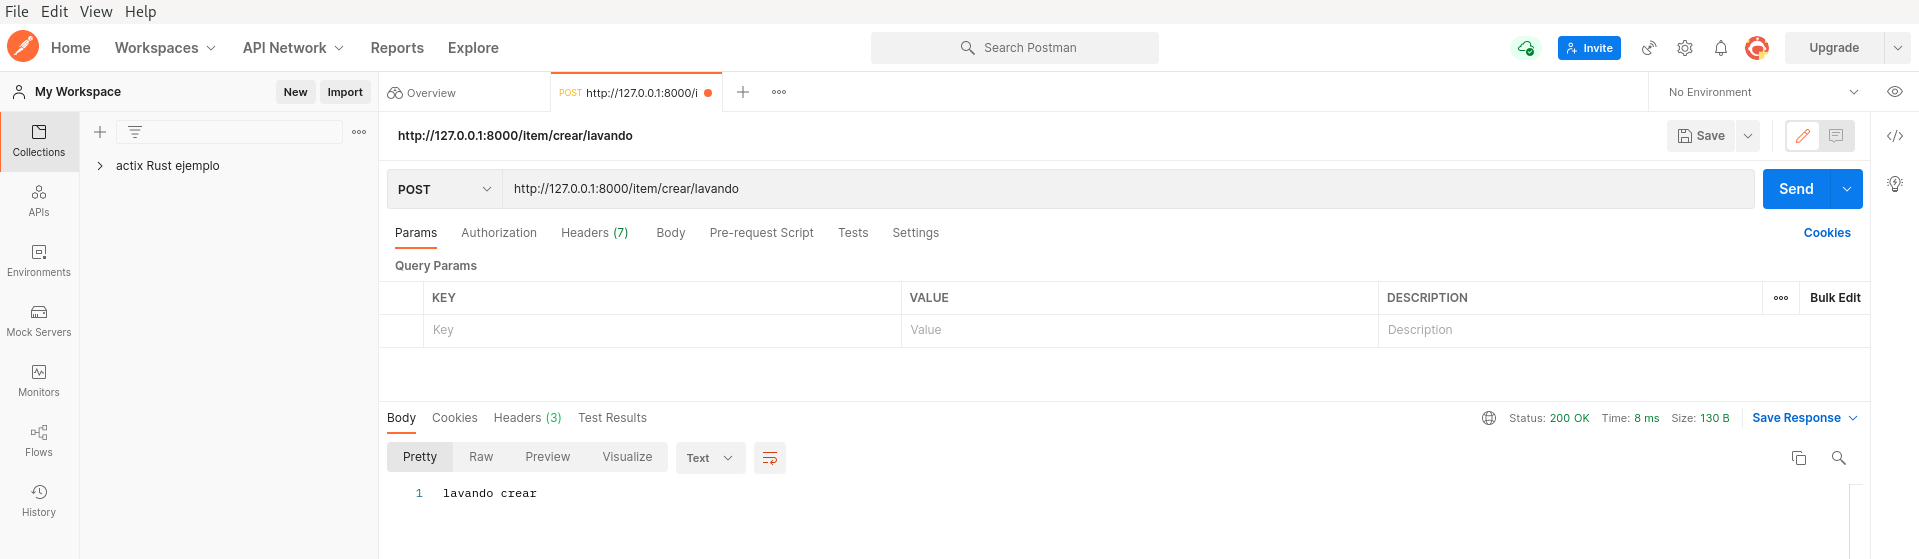
\includegraphics[width=1.0\textwidth]{capitulo3/postman_post.png}
	\caption{Revisando POST con postman}
	\label{cap3:003}
\end{figure}


Aquí, podemos ver que creamos un elemento de lavado para hacer con el mismo patrón de URL. Podemos ver que obtenemos un código 200 y luego una cadena creada por lavado en el cuerpo. La verificación de nuestro archivo de estado JSON nos muestra que el sistema aún funciona, ya que tenemos el código oxidado y lavado para hacer elementos, ambos pendientes. Podemos hacer que el mismo patrón de URL acepte los métodos POST y GET, simplemente llamando a la función de ruta dos veces en la fábrica de vistas pendientes con las funciones de publicación y obtención:

\begin{lstlisting}[language=C]
use actix_web::web;
mod crear;
use super::path::Path;

pub fn fabrica_item(app: &mut web::ServiceConfig) {
	let path_base: Path = Path{prefijo: String::from("/item")};
	app.route(&path_base.definir(String::from("/crear/{titulo}")),
	web::post().to(crear::crear));
	app.route(&path_base.definir(String::from("/crear/{titulo}")),
	web::get().to(crear::crear));
}
\end{lstlisting}


Teniendo en cuenta las diferencias que cubrimos anteriormente entre los métodos GET y POST, es sensato tener solo un método POST para nuestra función de creación.

Mirando hacia atrás en nuestra \textbf{GUI} de \textbf{Postman}, tenemos que pensar en el futuro. Con nuestra función de creación, una línea de texto es suficiente para decirnos que se ha creado el elemento. De hecho, ni siquiera tenemos que devolver nada en el cuerpo; el número de estado de devolución es suficiente para decirnos que el artículo ha sido creado. Sin embargo, cuando se trata de obtener una lista de tareas pendientes, necesitaremos datos estructurados. Para lograr esto, tendremos que serializar los datos \textbf{JSON} y devolvérnoslos.

\section{Uso de macros para la serialización JSON}

La serialización \textbf{JSON} se admite directamente a través de la crate \textbf{Actix-web}. Podemos demostrar esto creando una vista \textbf{GET} que devuelve todos nuestros elementos pendientes en el archivo \textbf{vistas/comercio/traer.rs}:

\begin{lstlisting}[language=C]
use actix_web::{web, Responder};
use serde_json::value::Value;
use serde_json::Map;
use crate::estado::leer_archivo;
pub async fn traer() -> impl Responder{
	let estado: Map<String, Value> = leer_archivo(String::from("./estado.json"));
	return web::Json(estado);
}
\end{lstlisting}

Aquí, simplemente leemos nuestro archivo JSON y lo devolvemos, lo pasamos a la estructura web::Json y luego lo devolvemos. La estructura web::Json implementa el rasgo Responder. Tenemos que definir esta nueva vista agregando la definición del módulo al archivo \textbf{vistas/comercial/mod.rs}, y luego agregar la definición de ruta a la función de fábrica:


\begin{lstlisting}[language=C]
mod traer
...
app.route(&path_base.definir(String::from("/traer")),
	web::get().to(traer::traer));
\end{lstlisting}

Ejecutar \textbf{http://127.0.0.1:8000/item/traer} nos brinda los siguientes datos JSON en el cuerpo de la respuesta:

\begin{lstlisting}[language=C]
{"code in rust":"pending","washing":"pending"}
\end{lstlisting}


Si bien esto hace el trabajo, no es flexible. Es posible que necesitemos dos listas diferentes: una para los elementos terminados y otra para los pendientes. También podrían querer un recuento de la cantidad de elementos y datos estructurados. Por ejemplo, es posible que necesitemos agregar una marca de tiempo para cuando se creó o terminó el elemento. Tener un cuerpo \textbf{JSON} simple para el elemento como título y tener el estado como valor no nos permite escalar la complejidad cuando sea necesario.

Para tener más control sobre el tipo de datos que vamos a devolver al usuario, vamos a tener que construir nuestras propias estructuras de serialización. Nuestra estructura de serialización presentará dos listas: una para artículos completados y otra para artículos pendientes. Estas listas se completarán con objetos que consisten en un título y un estado.

Como recordará nuestras estructuras de elementos \textbf{pendientes} y \textbf{Listos} se heredan a través de la composición de una estructura Base. Por lo tanto, tenemos que acceder al título y al estado desde la estructura \textbf{Base}. Sin embargo, nuestra estructura \textbf{Base} no es accesible al público. Tendremos que hacerlo accesible para que podamos serializar los atributos de cada elemento pendiente, como se muestra en la figura \ref{cap3:004}.


\begin{figure}[htb]
	\centering
	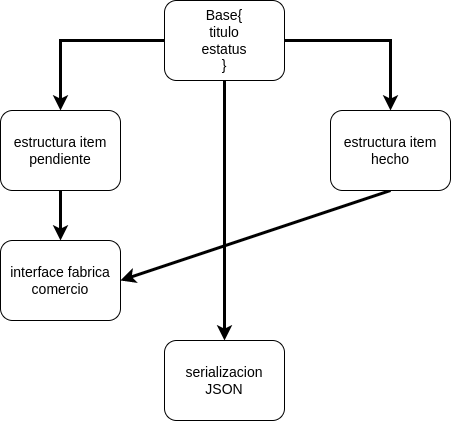
\includegraphics[width=0.6\textwidth]{capitulo3/estructura_comercio.png}
	\caption{Relación que tienen nuestras estructuras pendientes con nuestras interfaces}
	\label{cap3:004}
\end{figure}


Esto se puede hacer cambiando la declaración del módulo base en el archivo \textbf{comercio/estructuras/mod.rs} de \textbf{mod base;} a la base \textbf{mod pub;}. Ahora que la estructura \textbf{Base} está directamente disponible fuera del módulo, podemos construir nuestro propio módulo \textbf{json\_serialización} en el directorio \textbf{src} con la estructura de la figura \ref{cap3:005}.

\begin{figure}[htb]
	\centering
	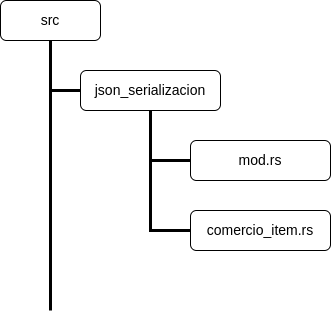
\includegraphics[width=0.4\textwidth]{capitulo3/serializacion.png}
	\caption{Estructura de serialización}
	\label{cap3:005}
\end{figure}


Nuestro nuevo módulo debe tener las siguientes dependencias agregadas al archivo \textbf{Cargo.toml}:

\begin{lstlisting}[language=C]
futures = "0.3.21"
serde = "1.0.136"
\end{lstlisting}

Ahora que tenemos todo, podemos definir un esquema JSON en nuestro archivo \textbf{src/json\_serializacion/comercio\_items.rs} y definir los parámetros y tipos para un cuerpo \textbf{JSON}:

\begin{lstlisting}[language=C]
use serde::Serialize;
use crate::comercio::TiposItem;
use crate::comercio::estructuras::base::Base;
#[derive(Serialize)]
pub struct ComercioItems {
	pub items_pendiente: Vec<Base>,
	pub items_hecho: Vec<Base>,
	pub contador_item_pendiente: i8,
	pub contador_item_hecho: i8
}
\end{lstlisting}

Aquí, todo lo que hemos hecho es definir una estructura pública estándar con parámetros. Luego usamos la macro de derivación para implementar el rasgo Serialize. Esto permite que los atributos de la estructura se serialicen en JSON con el nombre del atributo como clave. Por ejemplo, si la estructura \textbf{ComercioItems} tuviera un \textbf{contador\_item\_hecho} de uno, entonces el cuerpo \textbf{JSON} lo denotaría como \textbf{``contador\_item\_hecho'': 1}.

Ahora que se ha definido la serialización, tenemos que considerar el procesamiento de los datos. No sería escalable si tuviéramos que ordenar los datos y contarlos antes de llamar a la estructura. Esto agregaría código innecesario a la vista con respecto al procesamiento de datos para serialización en lugar de la lógica que pertenece a la vista en cuestión. También habilitaría el código duplicado. Solo habrá una forma de ordenar, contar y serializar los datos. Si otras vistas necesitaran devolver la lista de elementos, entonces tendríamos que duplicar el código nuevamente.

Teniendo esto en cuenta, tiene sentido construir un constructor para la estructura, donde ingerimos un vector de elementos pendientes, los clasificamos en los atributos correctos y luego los contamos:

\begin{lstlisting}[language=C]
impl ComercioItems {
	pub fn nuevo(items_entrada: Vec<TiposItem>) -> ComercioItems {
		let mut pendiente_array_buffer = Vec::new();
		let mut hecho_array_buffer = Vec::new();
		for item in items_entrada {
			match item {
				TiposItem::Pendiente(paquete) =>   pendiente_array_buffer.push(
				paquete.super_estructura),
				TiposItem::Hecho(paquete) => hecho_array_buffer.push(
				paquete.super_estructura)
			}
			let contar_hecho: i8 = hecho_array_buffer.len() as i8;
			let contar_pendiente: i8 = pendiente_array_buffer.len() as i8;
			return ComercioItems{
				items_pendiente: pendiente_array_buffer, contador_item_hecho: contar_hecho,
				contador_item_pendiente: contar_pendiente, items_hecho: hecho_array_buffer
			}
		}
	}
}
\end{lstlisting}

Lo que hacemos aquí es aceptar un vector de \textbf{TiposItem}. Luego los desempaquetamos con una declaración de coincidencia y los insertamos (agregamos) en el vector mutable correcto. Luego llamamos a la función \textbf{len} en cada vector. La función \textbf{len} devuelve un tamaño de uso, que es un tipo de entero sin signo del tamaño de un puntero. Debido a esto, lo proyectamos como un \textbf{i8} y luego redefinimos y devolvemos nuestra estructura, que está lista para serializarse en \textbf{JSON}.

Para utilizar nuestra estructura, tenemos que definirla en nuestra vista \textbf{TRAER}, en nuestro archivo \textbf{vistas/comercio/traer.rs}, y luego devolverlo:

\begin{lstlisting}[language=C]
use actix_web::{web, Responder};
use serde_json::value::Value;
use serde_json::Map;
use crate::estado::leer_archivo;
use crate::comercio::{TiposItem, fabrica_comercio};
use crate::serializacion_json::comercio_items::ComercioItems;

pub async fn traer() -> impl Responder {
	let estado: Map<String, Value> = leer_archivo("./estado.json");
	let mut array_buffer = Vec::new();
	for (key, value) in estado {
		let item_type: String = String::from(value.as_str().unwrap());
		let item: TiposItem = fabrica_comercio(&item_type, &key).unwrap();
		array_buffer.push(item);
	}
	let regresar_paquete: ComercioItems = ComercioItems::nuevo(array_buffer);
	return web::Json(regresar_paquete);
}
\end{lstlisting}

Aquí hay otro momento en el que todo encaja: usamos nuestra interfaz \textbf{leer\_archivo} para obtener el estado del archivo JSON. Luego recorremos el mapa, convirtiendo el tipo de elemento en una cadena y introduciéndolo en nuestra interfaz \textbf{fabrica\_comercio}. Una vez que tenemos el elemento construido de fábrica, lo agregamos a un vector y alimentamos ese vector en nuestra estructura de serialización JSON.

Para que nuestro módulo \textbf{serializacion\_json} funcione en nuestra aplicación, debemos declararlo en nuestro archivo \textbf{main.rs} con el \textbf{mod serializacion\_json}; línea de código. También tenemos que derivar la serialización en la estructura base en nuestro módulo \textbf{comercio} agregando la macro que definimos en nuestro archivo \textbf{src/comercio/estructuras/base.rs}, de la siguiente manera:

\begin{lstlisting}[language=C]
use serde::Serialize;

#[derive(Serialize)]
pub struct Base{
	pub titulo: String,
	pub estatus: String
}
impl Base {
	pub fn nuevo(titulo_entrada: &str, estatus_entrada: &str) -> Base {
		return Base {titulo: titulo_entrada.to_string(),
			estatus: estatus_entrada.to_string()}
	}
}
\end{lstlisting}

Esta es una respuesta limpia y bien estructurada que se puede ampliar y editar si es necesario a medida que se desarrolla nuestra aplicación. Podemos detenernos aquí, pero tenga en cuenta que nuestra vista \textbf{TRAER} devolvió una implementación del rasgo Responder. Esto significa que si nuestra estructura ComercioItems también implementa esto, se puede devolver directamente en una vista. Podemos hacer esto en nuestro archivo \textbf{serializacion\_json/comercio\_items.rs} con el siguiente bloque impl:


\begin{lstlisting}[language=C]
impl Responder for ComercioItems {
	type Error = Error;
	type Future = Ready<Result<HttpResponse, Error>>;
	fn respond_to(self, _req: &HttpRequest) -> Self::Future {
		let body = serde_json::to_string(&self).unwrap();
		ready(Ok(HttpResponse::Ok()
		.content_type("application/json")
		.body(body)))
	}
}

\end{lstlisting}

La función \textbf{respond\_to} se activa cuando se devuelve la función de vista. Aquí, devolvemos un tipo que nosotros mismos definimos llamado \textbf{Future}. Esto se compone de una estructura \textbf{Ready} del \textbf{crate de futuros}, lo que indica que el futuro está inmediatamente listo con un valor. Dentro de esto hay una estructura de resultado, que puede ser un error o una \textbf{HttpRequest}.

Serializamos la estructura propia usando \textbf{\&self} y la adjuntamos al cuerpo. Ahora, simplemente devolver nuestra estructura sin hacer ningún otro procesamiento en nuestra función \textbf{TRAER} se puede hacer creando un nuevo elemento pendiente y simplemente devolviéndolo. Esto se demuestra en el siguiente bloque de código:

\begin{lstlisting}[language=C]
let regresar_paquete: ComercioItems = ComercioItems::nuevo(array_buffer);
return regresar_paquete;
\end{lstlisting}

¡Esto nos da la misma respuesta que recibimos anteriormente! Ahora, estamos en el punto donde podemos refactorizar. Es razonable suponer que todas nuestras vistas de comercio requerirán una lista actualizada de comercio una vez finalizada la operación. Esta refactorización se puede realizar elevando todo el código de la función \textbf{TRAER} a una función llamada \textbf{regresar\_estado} en un archivo \textbf{utils} en el directorio \textbf{vistas/comercio/utils.rs} (recuerde definir el archivo en \textbf{mod.rs}). La función \textbf{regresar\_estado} devuelve la estructura \textbf{ComercioItems}. Esto luego acorta nuestra vista \textbf{TRAER} a lo siguiente:



